\documentclass[11pt]{article}
\usepackage[textwidth=18.0cm, textheight=23.0cm, top=2.0cm]{geometry}
\usepackage{pst-all}
\usepackage{amssymb}
\usepackage{tikz}
\usepackage{underscore}\begin{document}
\pagestyle{empty}


ClassName: \underline{\textbf{Class_05.2bp-10}}
\par
BinSize: \underline{\textbf{100 × 100}}
\par
ReduceSize: \underline{\textbf{100 × 100}}
\par
TypeNum: \underline{\textbf{40}}
\par
Num: \underline{\textbf{40}}
\par
OutS: \underline{\textbf{80000}}
\par
InS: \underline{\textbf{69519}}
\par
Rate: \underline{\textbf{0.869}}
\par
UB: \underline{\textbf{8}}
\par
LB0: \underline{\textbf{8}}
\par
LB: \underline{\textbf{8}}
\par
LBWithCut: \underline{\textbf{8}}
\par
NodeCut: \underline{\textbf{0}}
\par
ExtendedNodeCnt: \underline{\textbf{1}}
\par
GenNodeCnt: \underline{\textbf{1}}
\par
PrimalNode: \underline{\textbf{0}}
\par
ColumnCount: \underline{\textbf{8}}
\par
TotalCutCount: \underline{\textbf{0}}
\par
RootCutCount: \underline{\textbf{0}}
\par
LPSolverCnt: \underline{\textbf{1}}
\par
PricingSolverCnt: \underline{\textbf{0}}
\par
BranchAndBoundNum: \underline{\textbf{1}}
\par
isOpt: \underline{\textbf{true}}
\par
TimeOnInitSolution: \underline{\textbf{0.020 s}}
\par
TimeOnPrimal: \underline{\textbf{0.000 s}}
\par
TimeOnPricing: \underline{\textbf{0.000 s}}
\par
TimeOnRmp: \underline{\textbf{0.063 s}}
\par
TotalTime: \underline{\textbf{0.145 s}}
\par
\newpage


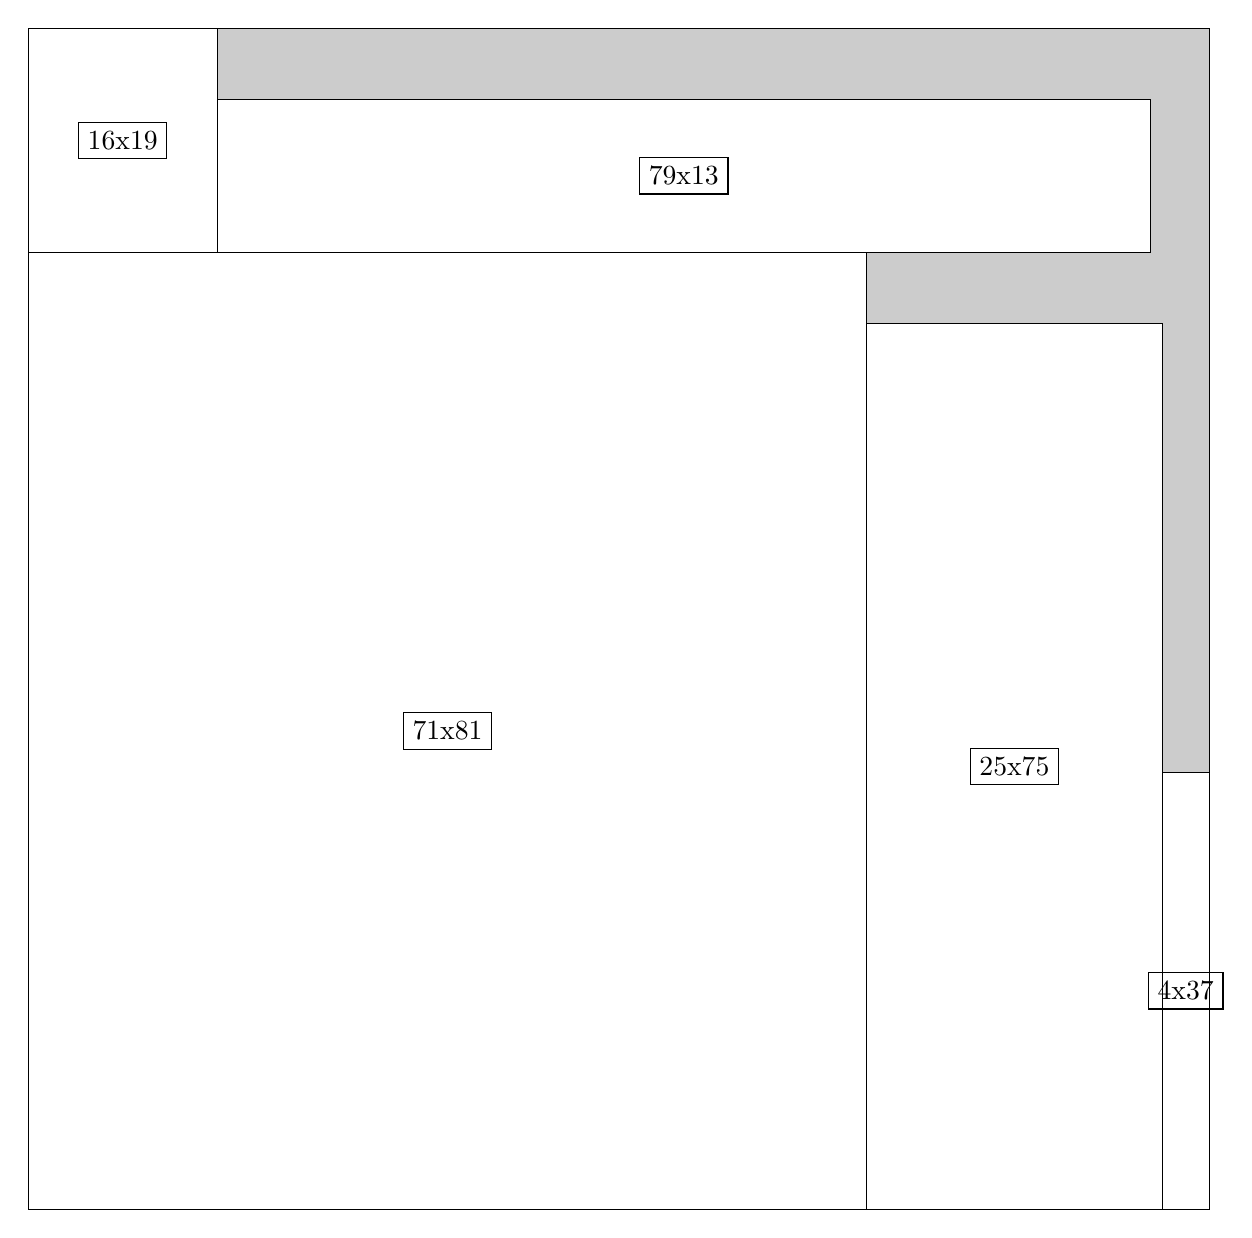
\begin{tikzpicture}[shorten >=1pt,scale=1.0,every node/.style={scale=1.0},->]
\tikzstyle{vertex}=[circle,fill=black!25,minimum size=14pt,inner sep=0pt]
\filldraw[fill=gray!40!white, draw=black] (0,0) rectangle (15.0,15.0);
\foreach \name/\x/\y/\w/\h in {71x81/0.0/0.0/10.65/12.15,25x75/10.65/0.0/3.75/11.25,79x13/2.4/12.15/11.85/1.95,16x19/0.0/12.15/2.4/2.85,4x37/14.399999999999999/0.0/0.6/5.55}
\filldraw[fill=white!40!white, draw=black] (\x,\y) rectangle node[draw] (\name) {\name} ++(\w,\h);
\end{tikzpicture}


w =71 , h =81 , x =0 , y =0 , v =5751
\par
w =25 , h =75 , x =71 , y =0 , v =1875
\par
w =79 , h =13 , x =16 , y =81 , v =1027
\par
w =16 , h =19 , x =0 , y =81 , v =304
\par
w =4 , h =37 , x =96 , y =0 , v =148
\par
\newpage


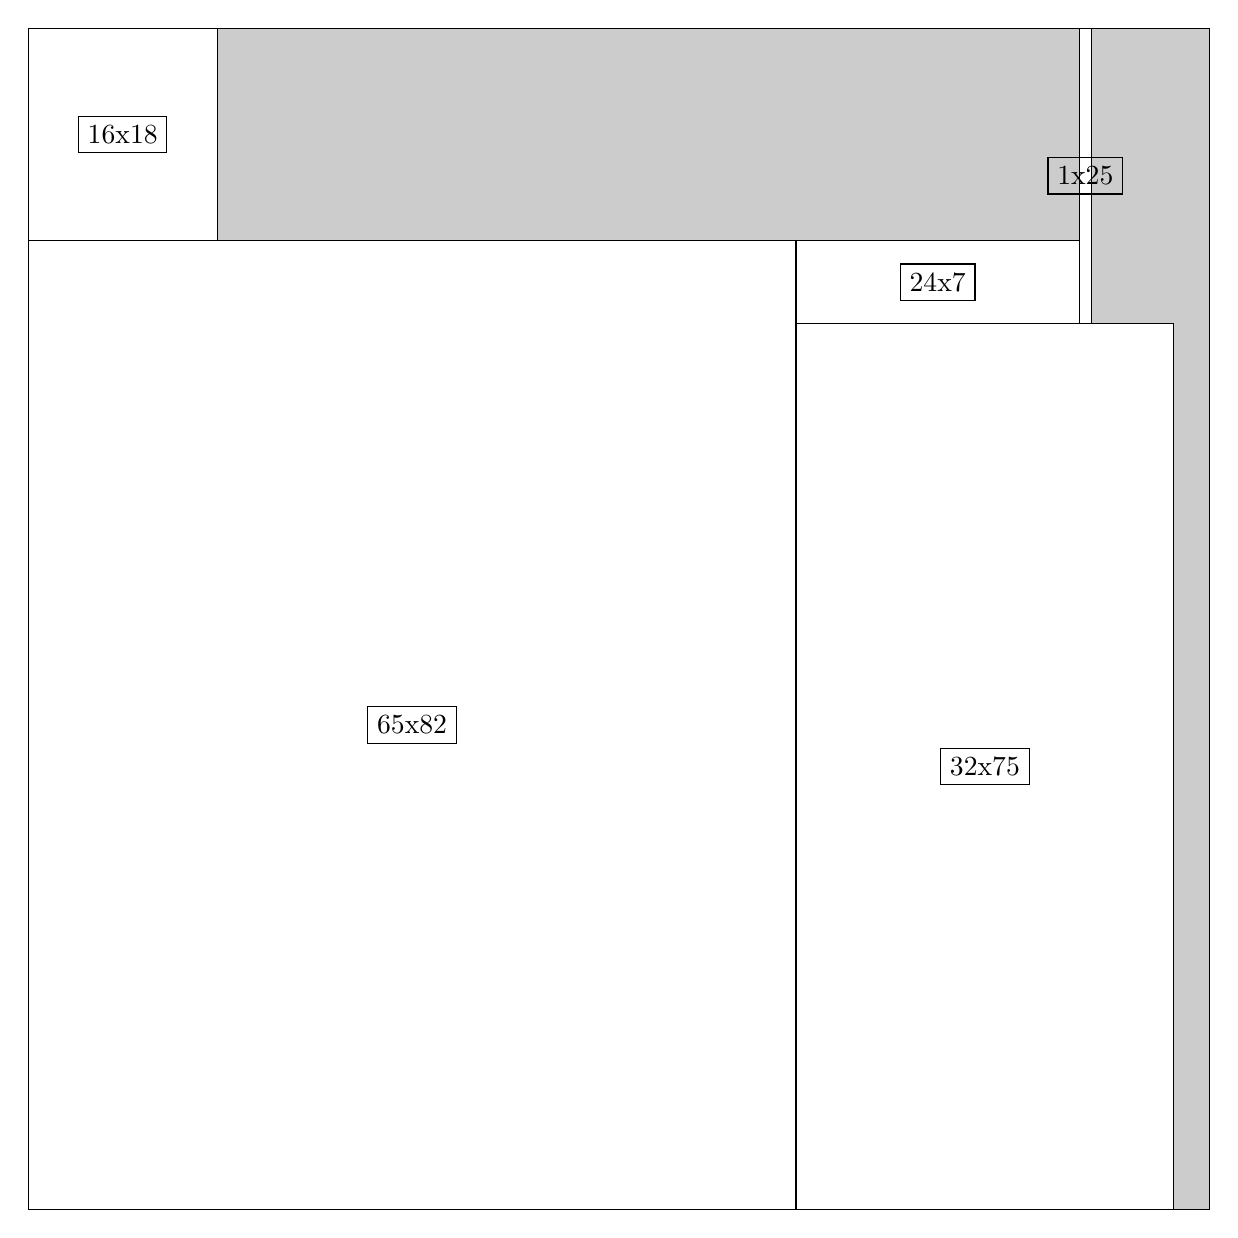
\begin{tikzpicture}[shorten >=1pt,scale=1.0,every node/.style={scale=1.0},->]
\tikzstyle{vertex}=[circle,fill=black!25,minimum size=14pt,inner sep=0pt]
\filldraw[fill=gray!40!white, draw=black] (0,0) rectangle (15.0,15.0);
\foreach \name/\x/\y/\w/\h in {65x82/0.0/0.0/9.75/12.299999999999999,32x75/9.75/0.0/4.8/11.25,16x18/0.0/12.299999999999999/2.4/2.6999999999999997,24x7/9.75/11.25/3.5999999999999996/1.05,1x25/13.35/11.25/0.15/3.75}
\filldraw[fill=white!40!white, draw=black] (\x,\y) rectangle node[draw] (\name) {\name} ++(\w,\h);
\end{tikzpicture}


w =65 , h =82 , x =0 , y =0 , v =5330
\par
w =32 , h =75 , x =65 , y =0 , v =2400
\par
w =16 , h =18 , x =0 , y =82 , v =288
\par
w =24 , h =7 , x =65 , y =75 , v =168
\par
w =1 , h =25 , x =89 , y =75 , v =25
\par
\newpage


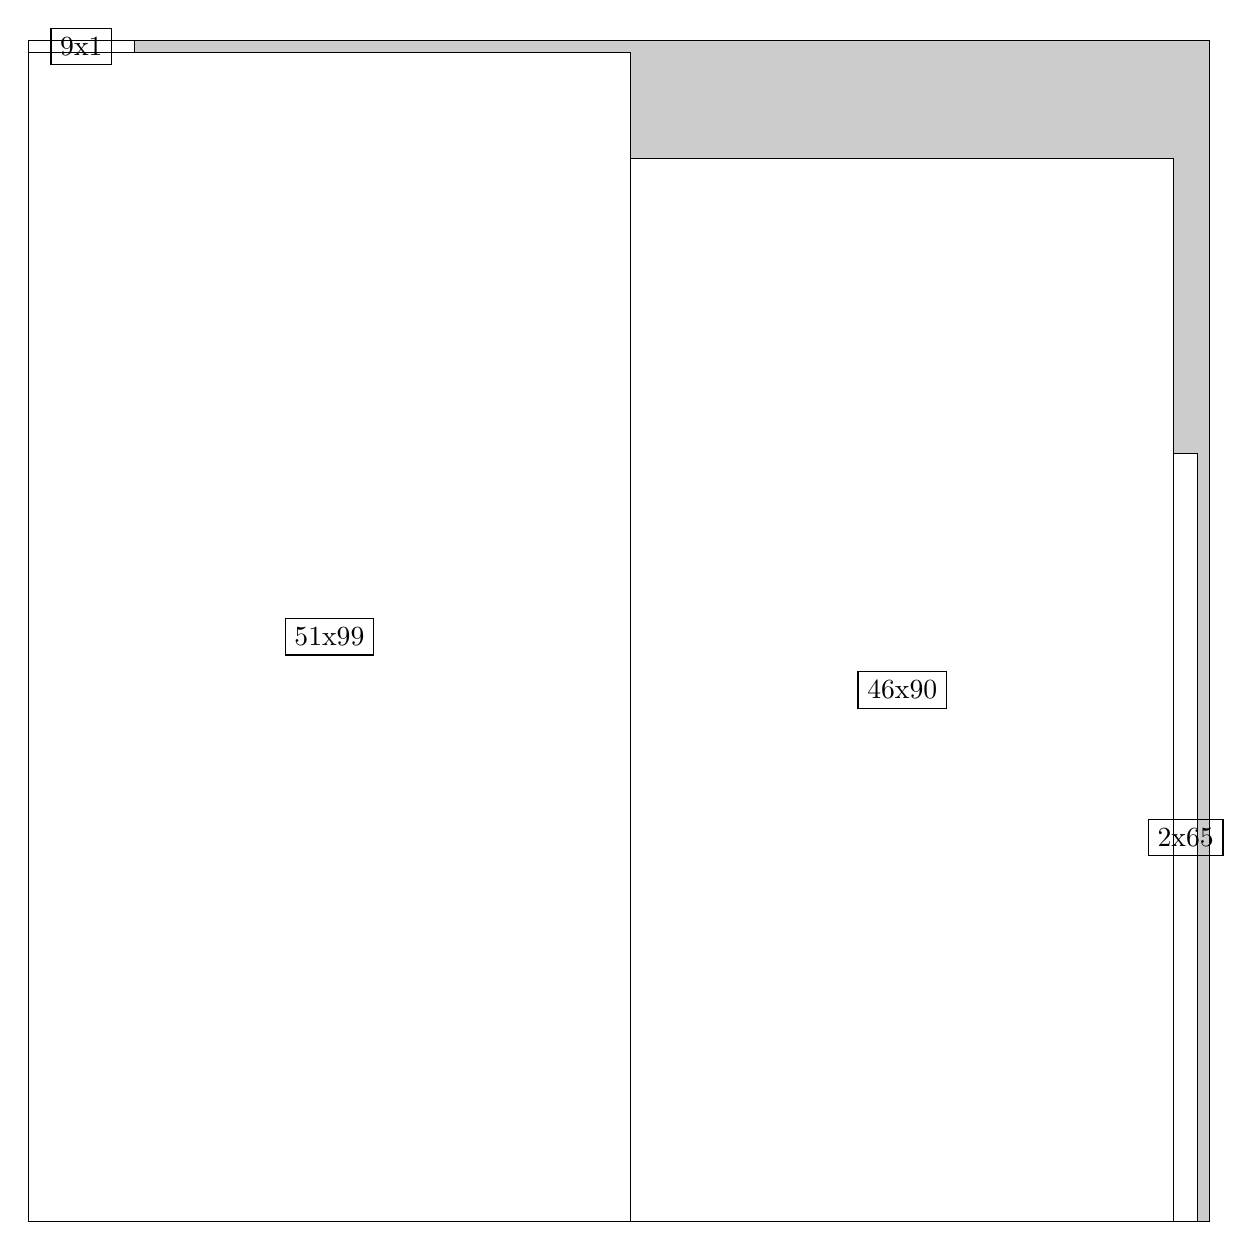
\begin{tikzpicture}[shorten >=1pt,scale=1.0,every node/.style={scale=1.0},->]
\tikzstyle{vertex}=[circle,fill=black!25,minimum size=14pt,inner sep=0pt]
\filldraw[fill=gray!40!white, draw=black] (0,0) rectangle (15.0,15.0);
\foreach \name/\x/\y/\w/\h in {51x99/0.0/0.0/7.6499999999999995/14.85,46x90/7.6499999999999995/0.0/6.8999999999999995/13.5,2x65/14.549999999999999/0.0/0.3/9.75,9x1/0.0/14.85/1.3499999999999999/0.15}
\filldraw[fill=white!40!white, draw=black] (\x,\y) rectangle node[draw] (\name) {\name} ++(\w,\h);
\end{tikzpicture}


w =51 , h =99 , x =0 , y =0 , v =5049
\par
w =46 , h =90 , x =51 , y =0 , v =4140
\par
w =2 , h =65 , x =97 , y =0 , v =130
\par
w =9 , h =1 , x =0 , y =99 , v =9
\par
\newpage


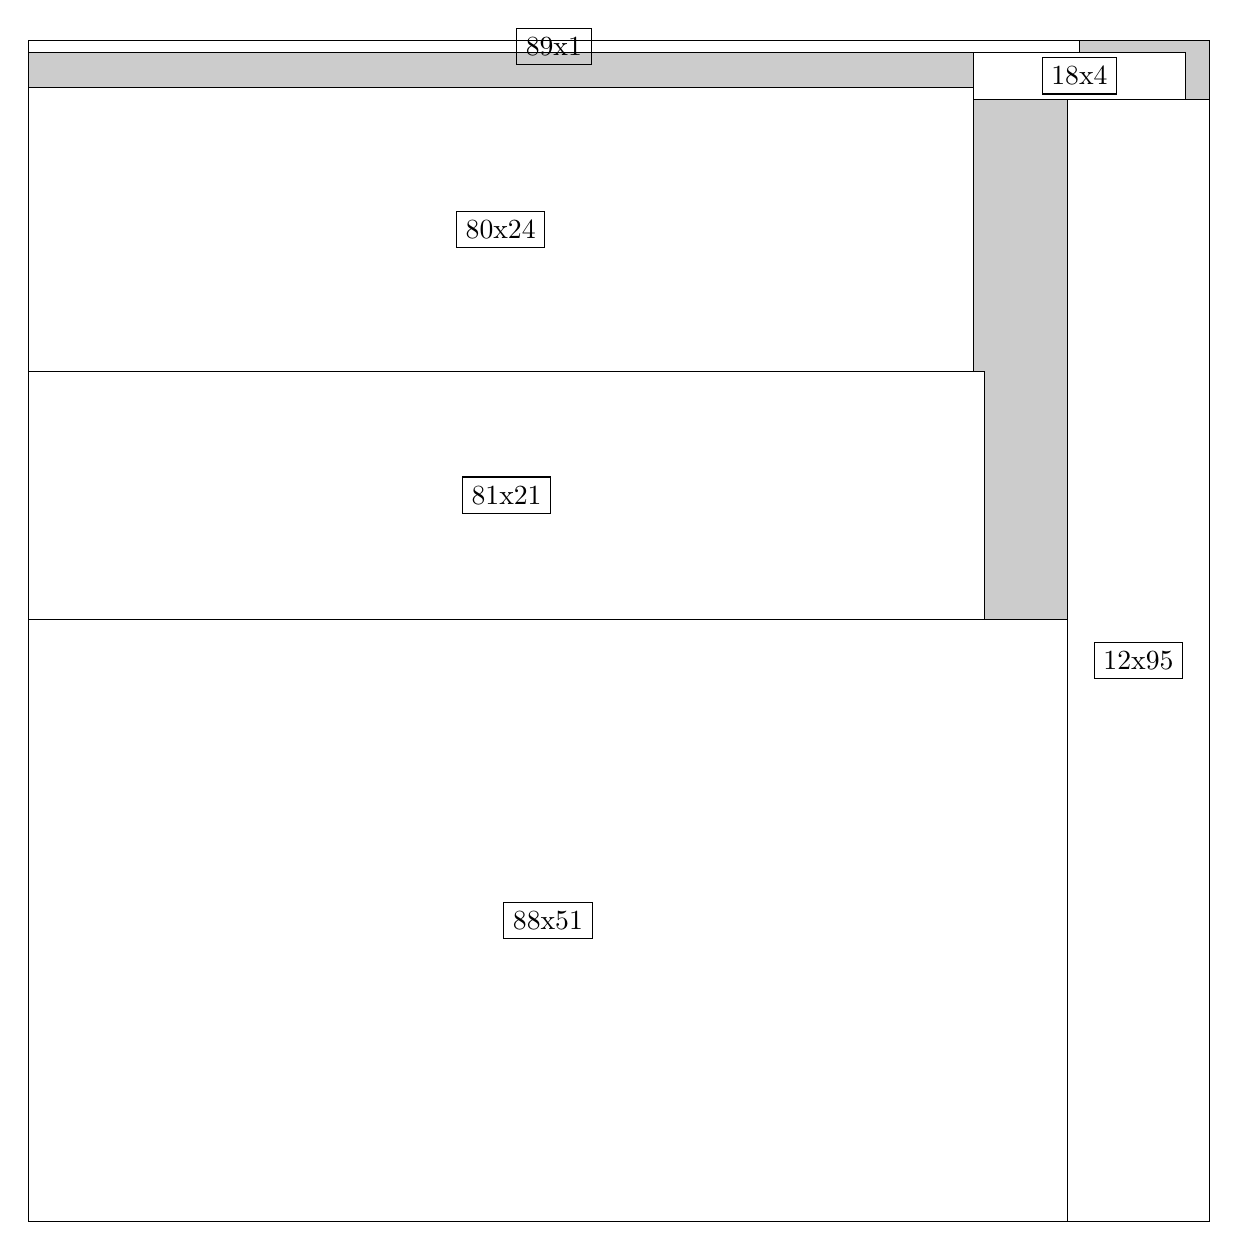
\begin{tikzpicture}[shorten >=1pt,scale=1.0,every node/.style={scale=1.0},->]
\tikzstyle{vertex}=[circle,fill=black!25,minimum size=14pt,inner sep=0pt]
\filldraw[fill=gray!40!white, draw=black] (0,0) rectangle (15.0,15.0);
\foreach \name/\x/\y/\w/\h in {88x51/0.0/0.0/13.2/7.6499999999999995,81x21/0.0/7.6499999999999995/12.15/3.15,80x24/0.0/10.799999999999999/12.0/3.5999999999999996,12x95/13.2/0.0/1.7999999999999998/14.25,89x1/0.0/14.85/13.35/0.15,18x4/12.0/14.25/2.6999999999999997/0.6}
\filldraw[fill=white!40!white, draw=black] (\x,\y) rectangle node[draw] (\name) {\name} ++(\w,\h);
\end{tikzpicture}


w =88 , h =51 , x =0 , y =0 , v =4488
\par
w =81 , h =21 , x =0 , y =51 , v =1701
\par
w =80 , h =24 , x =0 , y =72 , v =1920
\par
w =12 , h =95 , x =88 , y =0 , v =1140
\par
w =89 , h =1 , x =0 , y =99 , v =89
\par
w =18 , h =4 , x =80 , y =95 , v =72
\par
\newpage


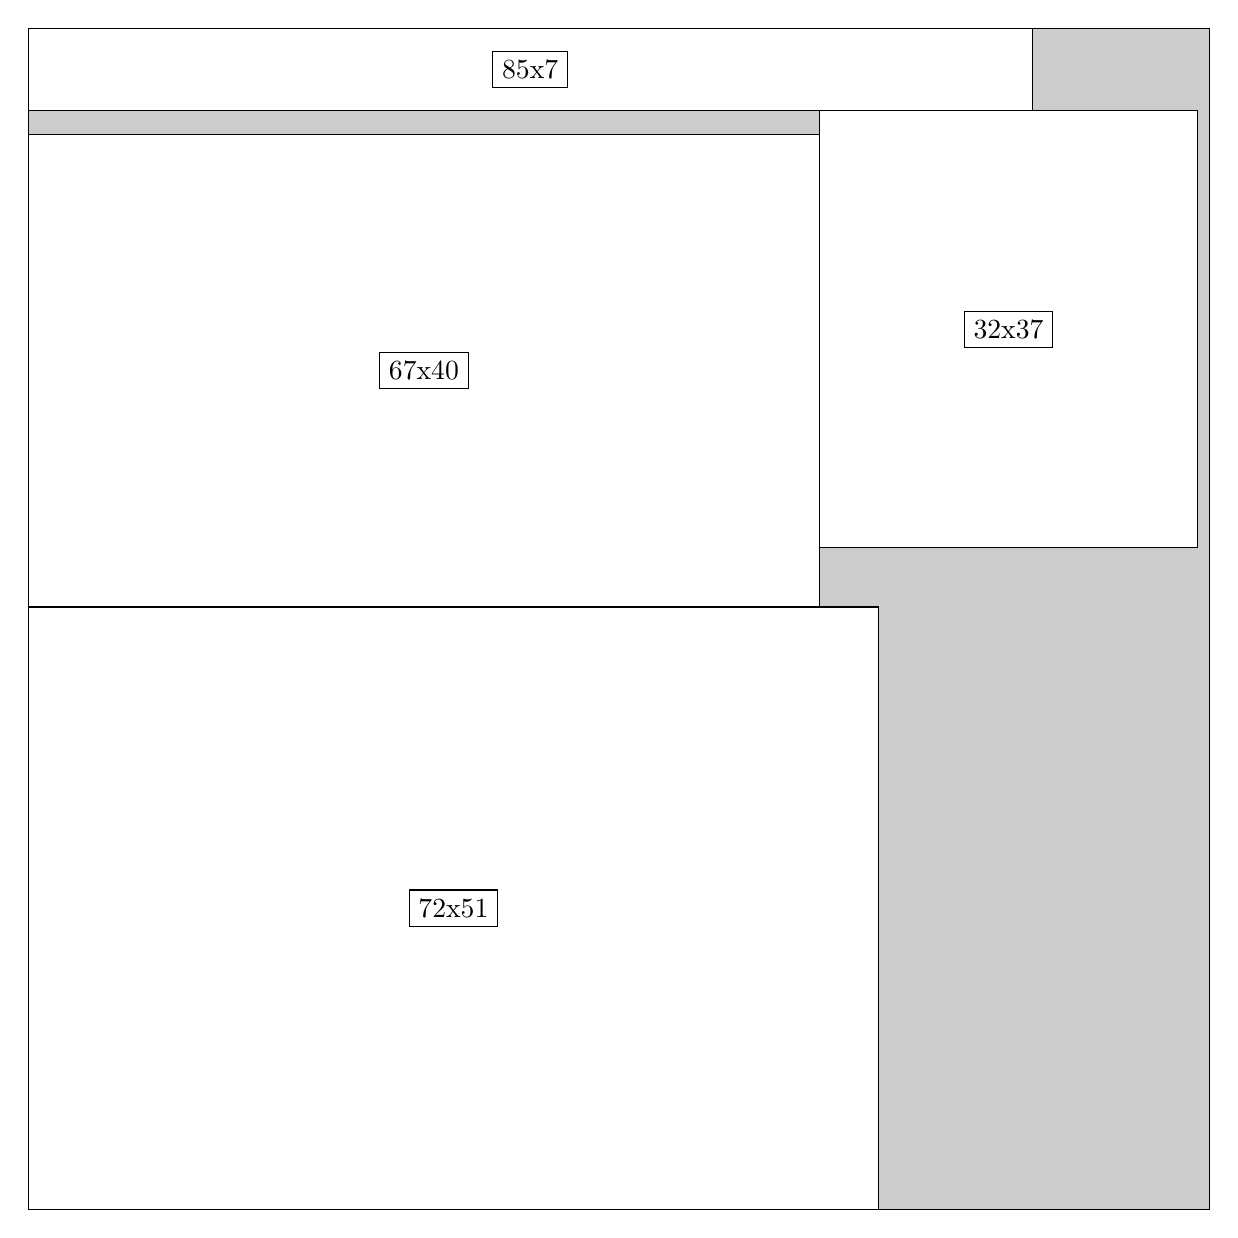
\begin{tikzpicture}[shorten >=1pt,scale=1.0,every node/.style={scale=1.0},->]
\tikzstyle{vertex}=[circle,fill=black!25,minimum size=14pt,inner sep=0pt]
\filldraw[fill=gray!40!white, draw=black] (0,0) rectangle (15.0,15.0);
\foreach \name/\x/\y/\w/\h in {72x51/0.0/0.0/10.799999999999999/7.6499999999999995,67x40/0.0/7.6499999999999995/10.049999999999999/6.0,32x37/10.049999999999999/8.4/4.8/5.55,85x7/0.0/13.95/12.75/1.05}
\filldraw[fill=white!40!white, draw=black] (\x,\y) rectangle node[draw] (\name) {\name} ++(\w,\h);
\end{tikzpicture}


w =72 , h =51 , x =0 , y =0 , v =3672
\par
w =67 , h =40 , x =0 , y =51 , v =2680
\par
w =32 , h =37 , x =67 , y =56 , v =1184
\par
w =85 , h =7 , x =0 , y =93 , v =595
\par
\newpage


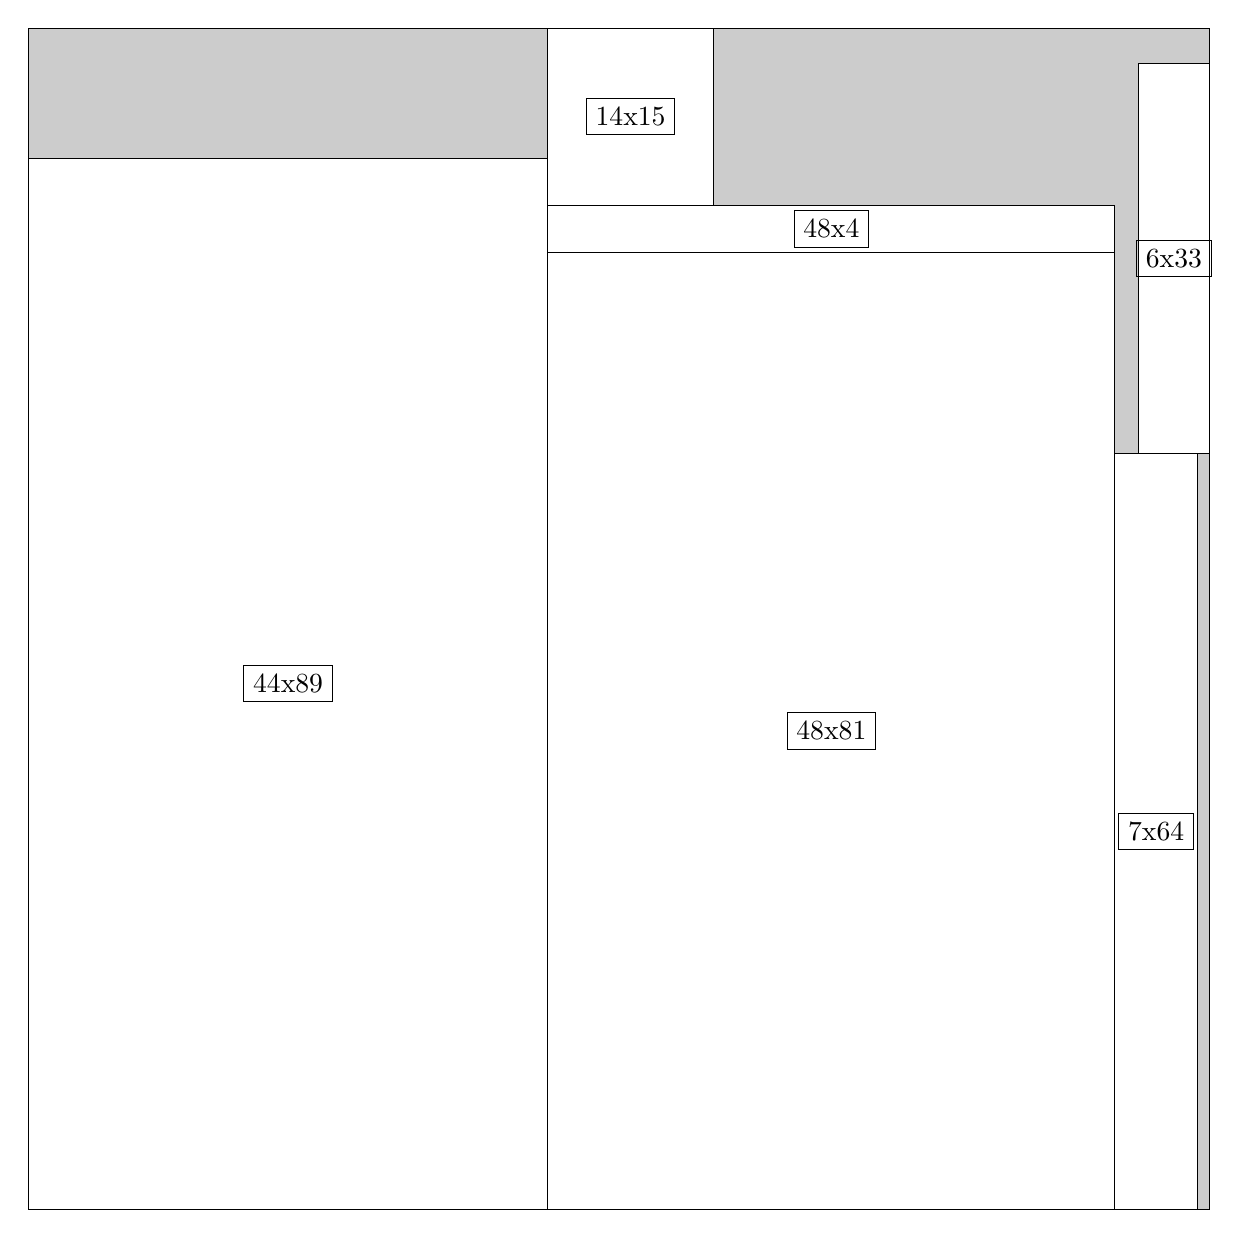
\begin{tikzpicture}[shorten >=1pt,scale=1.0,every node/.style={scale=1.0},->]
\tikzstyle{vertex}=[circle,fill=black!25,minimum size=14pt,inner sep=0pt]
\filldraw[fill=gray!40!white, draw=black] (0,0) rectangle (15.0,15.0);
\foreach \name/\x/\y/\w/\h in {44x89/0.0/0.0/6.6/13.35,48x81/6.6/0.0/7.199999999999999/12.15,7x64/13.799999999999999/0.0/1.05/9.6,14x15/6.6/12.75/2.1/2.25,6x33/14.1/9.6/0.8999999999999999/4.95,48x4/6.6/12.15/7.199999999999999/0.6}
\filldraw[fill=white!40!white, draw=black] (\x,\y) rectangle node[draw] (\name) {\name} ++(\w,\h);
\end{tikzpicture}


w =44 , h =89 , x =0 , y =0 , v =3916
\par
w =48 , h =81 , x =44 , y =0 , v =3888
\par
w =7 , h =64 , x =92 , y =0 , v =448
\par
w =14 , h =15 , x =44 , y =85 , v =210
\par
w =6 , h =33 , x =94 , y =64 , v =198
\par
w =48 , h =4 , x =44 , y =81 , v =192
\par
\newpage


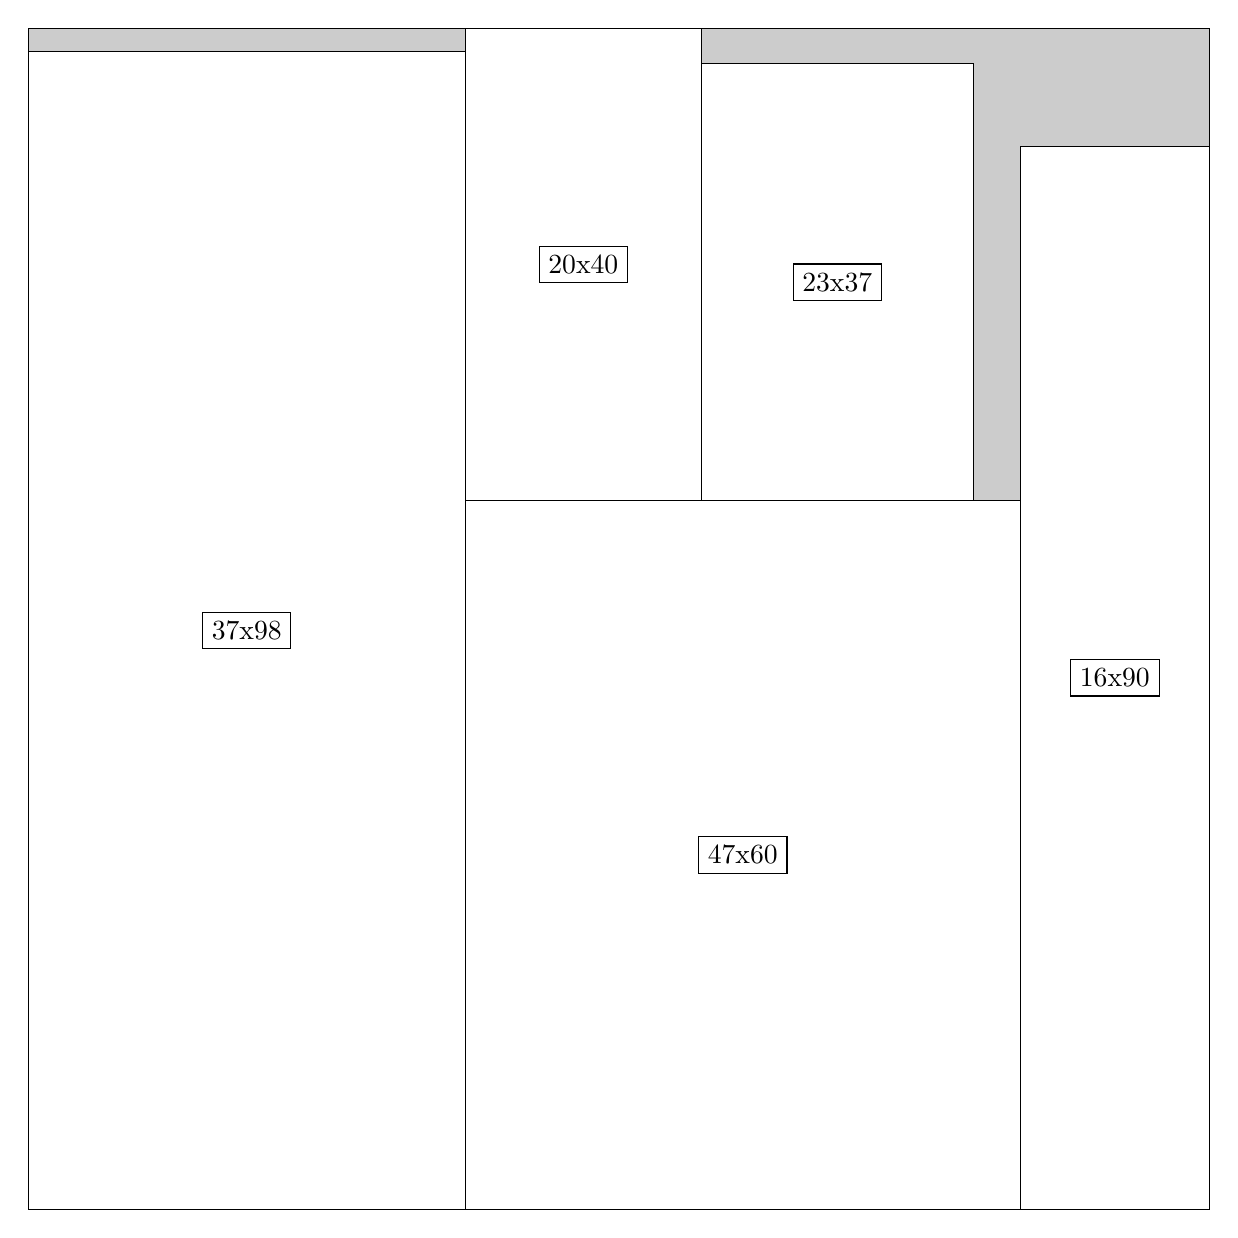
\begin{tikzpicture}[shorten >=1pt,scale=1.0,every node/.style={scale=1.0},->]
\tikzstyle{vertex}=[circle,fill=black!25,minimum size=14pt,inner sep=0pt]
\filldraw[fill=gray!40!white, draw=black] (0,0) rectangle (15.0,15.0);
\foreach \name/\x/\y/\w/\h in {37x98/0.0/0.0/5.55/14.7,47x60/5.55/0.0/7.05/9.0,16x90/12.6/0.0/2.4/13.5,23x37/8.549999999999999/9.0/3.4499999999999997/5.55,20x40/5.55/9.0/3.0/6.0}
\filldraw[fill=white!40!white, draw=black] (\x,\y) rectangle node[draw] (\name) {\name} ++(\w,\h);
\end{tikzpicture}


w =37 , h =98 , x =0 , y =0 , v =3626
\par
w =47 , h =60 , x =37 , y =0 , v =2820
\par
w =16 , h =90 , x =84 , y =0 , v =1440
\par
w =23 , h =37 , x =57 , y =60 , v =851
\par
w =20 , h =40 , x =37 , y =60 , v =800
\par
\newpage


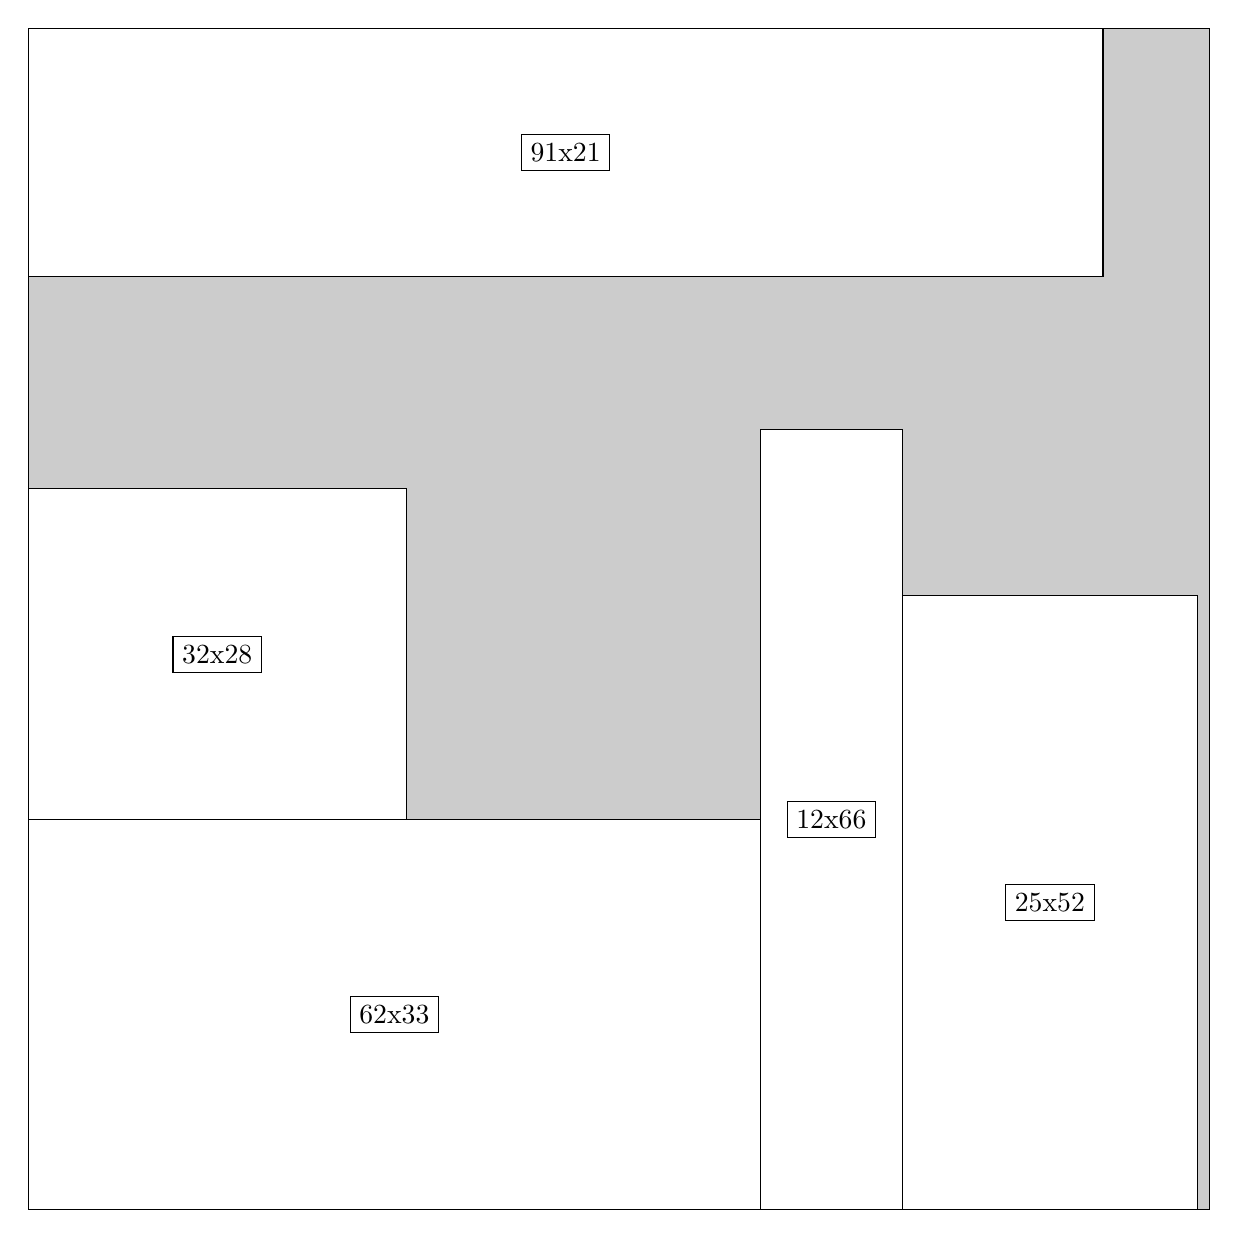
\begin{tikzpicture}[shorten >=1pt,scale=1.0,every node/.style={scale=1.0},->]
\tikzstyle{vertex}=[circle,fill=black!25,minimum size=14pt,inner sep=0pt]
\filldraw[fill=gray!40!white, draw=black] (0,0) rectangle (15.0,15.0);
\foreach \name/\x/\y/\w/\h in {62x33/0.0/0.0/9.299999999999999/4.95,25x52/11.1/0.0/3.75/7.8,91x21/0.0/11.85/13.65/3.15,32x28/0.0/4.95/4.8/4.2,12x66/9.299999999999999/0.0/1.7999999999999998/9.9}
\filldraw[fill=white!40!white, draw=black] (\x,\y) rectangle node[draw] (\name) {\name} ++(\w,\h);
\end{tikzpicture}


w =62 , h =33 , x =0 , y =0 , v =2046
\par
w =25 , h =52 , x =74 , y =0 , v =1300
\par
w =91 , h =21 , x =0 , y =79 , v =1911
\par
w =32 , h =28 , x =0 , y =33 , v =896
\par
w =12 , h =66 , x =62 , y =0 , v =792
\par
\newpage


\end{document}